

\documentclass{article}
\usepackage[utf8]{inputenc}
\usepackage[utf8]{inputenc}
\usepackage[T1]{fontenc}
\usepackage[english]{babel}
\usepackage{fullpage}
\usepackage{color}
\usepackage[table]{xcolor}
\usepackage{listings}
 
\definecolor{darkWhite}{rgb}{0.94,0.94,0.94}
 
\lstset{
  aboveskip=3mm,
  belowskip=-2mm,
  backgroundcolor=\color{darkWhite},
  basicstyle=\footnotesize,
  breakatwhitespace=false,
  breaklines=true,
  captionpos=b,
  commentstyle=\color{red},
  deletekeywords={...},
  escapeinside={\%*}{*)},
  extendedchars=true,
  framexleftmargin=16pt,
  framextopmargin=3pt,
  framexbottommargin=6pt,
  frame=tb,
  keepspaces=true,
  keywordstyle=\color{blue},
  language=C,
  literate=
  {²}{{\textsuperscript{2}}}1
  {⁴}{{\textsuperscript{4}}}1
  {⁶}{{\textsuperscript{6}}}1
  {⁸}{{\textsuperscript{8}}}1
  {€}{{\euro{}}}1
  {é}{{\'e}}1
  {è}{{\`{e}}}1
  {ê}{{\^{e}}}1
  {ë}{{\¨{e}}}1
  {É}{{\'{E}}}1
  {Ê}{{\^{E}}}1
  {û}{{\^{u}}}1
  {ù}{{\`{u}}}1
  {â}{{\^{a}}}1
  {à}{{\`{a}}}1
  {á}{{\'{a}}}1
  {ã}{{\~{a}}}1
  {Á}{{\'{A}}}1
  {Â}{{\^{A}}}1
  {Ã}{{\~{A}}}1
  {ç}{{\c{c}}}1
  {Ç}{{\c{C}}}1
  {õ}{{\~{o}}}1
  {ó}{{\'{o}}}1
  {ô}{{\^{o}}}1
  {Õ}{{\~{O}}}1
  {Ó}{{\'{O}}}1
  {Ô}{{\^{O}}}1
  {î}{{\^{i}}}1
  {Î}{{\^{I}}}1
  {í}{{\'{i}}}1
  {Í}{{\~{Í}}}1,
  morekeywords={*,...},
  numbers=left,
  numbersep=10pt,
  numberstyle=\tiny\color{black},
  rulecolor=\color{black},
  showspaces=false,
  showstringspaces=false,
  showtabs=false,
  stepnumber=1,
  stringstyle=\color{gray},
  tabsize=4,
  title=\lstname,
}
\usepackage{graphicx}
\graphicspath{ {./images/} }
\title{HAI804I – Analyse et Traitement d'Images}
\author{Fabien Caballero }

\begin{document}  

\maketitle
    \tableofcontents

\newpage

\begin{figure}[h]
\centerline{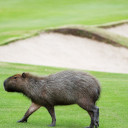
\includegraphics[scale=4]{./rendus/capybaral.jpg}  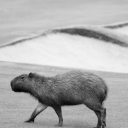
\includegraphics[scale=0.953]{./rendus/capybatap.png}}
\caption{Image d'origine utilisée le long du TP en pgm et en ppm}
\end{figure}

\section{Seuillage d'une image au format pgm}


\begin{figure}[h]
\centerline{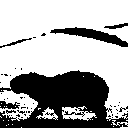
\includegraphics[scale=1.4]{./rendus/capybatapSeuil.png}}
\caption{capybara.pgm avec un seuil automatique avec la moyenne}
\end{figure}

Pour le seuillage, on parcours chaque pixel et on teste sa valeur, si celle-ci est inférieure au seuil on met à 0 (noir) ce pixel dans le tableau de l'image de sortie, sinon à 255 (blanc).

\newpage
\section{Érosion et dilatation }
\subsection{Érosion}

L'érosion permet d'éliminer les morceux d'objet qui appartiennent en fait au fond.
Pour éroder une image on parcours chaque pixel, et pour chacun d'eux on regarde dans ses voisins selon l'élément structurant et si un de ses voisins appartient au fond alors le pixel courant est défini comme appartenant au fond.
Il faut faire attention de bien utiliser une image de lecture et une autre d'écriture différente l'une de l'autre.

\begin{figure}[h]
\centerline{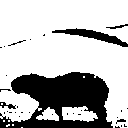
\includegraphics[scale=1.4]{./rendus/capybatapEro.png}}
\caption{capybara.pgm Seuillée puis érodée}
\end{figure}

\subsection{Dilatation}
La dilatation est exactement comme une érosion à la seule différence qu'elle comble les trous dans l'objet, elle va donc augmenter le nombre de pixels appartenant à l'objet.

Donc lors de la comparaison avec ses voisins on regarde si l'un de ses voisins appartient à l'objet et si c'est le cas le pixel courant va être défini comme appartenant à l'objet.


\begin{figure}[h]
\centerline{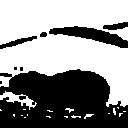
\includegraphics[scale=1.4]{./rendus/capybatapDila.png}}
\caption{capybara.pgm seuillée puis dilatée}
\end{figure}

\newpage
\section{Fermeture et Ouverture}
\subsection{Fermeture}
La fermeture est le fait d'appliquer une dilatation et sur le résultat appliquer une érosion.
Cela permet de recoller des morceaux d'objet proches de manière à fermer les contours disjoints, et les lisser.

\begin{figure}[h]
\centerline{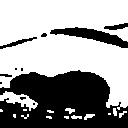
\includegraphics[scale=1.4]{./rendus/capybatapferm.png}}
\caption{capybara.pgm seuillée puis fermée}
\end{figure}


\subsection{Ouverture}
L'ouverture est le fait d'appliquer une érosion et sur le résultat appliquer une dilatation.
Cela permet d'isoler les objets présents dans l'image, et lisser les contours.

\begin{figure}[h]
\centerline{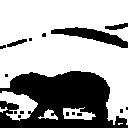
\includegraphics[scale=1.4]{./rendus/capybatapouv.png}}
\caption{capybara.pgm seuillée puis ouverte}
\end{figure}

\newpage
\subsection{Fermeture puis Ouverture}
Application d'une fermeture puis sur le résultat une ouverture.
\begin{figure}[h]
\centerline{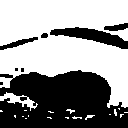
\includegraphics[scale=1.4]{./rendus/capybatapfermouv.png}}
\caption{capybara.pgm seuillée puis fermée et ouverte}
\end{figure}

\newpage
\section{3 dilatations, 6 érosions et 3 dilatations}
On enchaîne 3 dilatations puis 6 érosions et de nouveau 3 dilatations en 12 étapes différentes.
À chaque fois le résultat de l'action et l'entrée de la suivante.
\begin{figure}[h]
\centerline{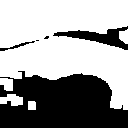
\includegraphics[scale=1.4]{./rendus/capybatap363.png}}
\caption{capaybara.pgm seuillée puis enchaînement de 3 dilatations, 6 érosions et 3 dilatations}
\end{figure}

Puis en une seule fois avec un seul programme qui fait directement les 12 actions précédentes.
\begin{figure}[h]
\centerline{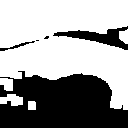
\includegraphics[scale=1.4]{./rendus/capybatap363.png}}
\caption{capaybara.pgm seuillée puis enchaînement de 3 dilatations, 6 érosions et 3 dilatations en 1 programme}
\end{figure}

On constate que le résultat est le même.

\newpage
\section{Segmentation}
La segmentation permet de faire apparaître les contours des objets.
Pour cela on prend l'image érodée et l'image dilatée et on fait le XOR entre chaque pixel, lorsque les valeurs sont identiques on défini le pixel de l'image de sortie à noir dès qu'ils sont différents à blanc.
En effet, étant donné que la dilatation agrandie la surface de l'objet  et que l'érosion la réduit il va y avoir des pixels qui vont être différents sur les bords des objets, avec le XOR, cela va donner les contours.
 \begin{figure}[h]
\centerline{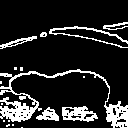
\includegraphics[scale=1.4]{./rendus/capybatapSegment.png}}
\caption{Segmentation de capybara.pgm seuillée} 
\end{figure}

\newpage
\section{Dilatation, Erosion, Fermeture et Ouverture pour une image pgm}

On applique le même algo que pour une image seuillée sauf que au lieu de regarder si il a un voisin à 0 ou à 255 on va prendre le min ou le max.
On utilise le min lors d'une érosion et le max lors d'une dilatation.

\begin{figure}[h]
\centerline{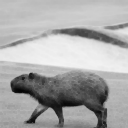
\includegraphics[scale=1.4]{./rendus/ErosionGrey.png}}
\caption{Erosion de capybara.pgm}
\end{figure}

\begin{figure}[h]
\centerline{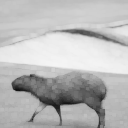
\includegraphics[scale=1.4]{./rendus/DilatationGrey.png}}
\caption{Dilatation de capybara.pgm}
\end{figure}

\begin{figure}[h]
\centerline{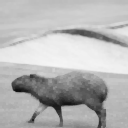
\includegraphics[scale=1.4]{./rendus/FermetureGrey.png}}
\caption{Fermeture de capybara.pgm}
\end{figure}

\begin{figure}
\centerline{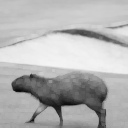
\includegraphics[scale=1.4]{./rendus/OuvertureGrey.png}}
\caption{Ouverture de capybara.pgm}
\end{figure}


\newpage
\section{Dilatation, Erosion, Fermeture et Ouverture pour une image ppm}

Pour une image en couleur il faut séparer chaque composante faire l'action voulue comme s'il s'agissait d'une image en niveaux de gris, puis de re-assembler les composantes.

\begin{figure}[h]
\centerline{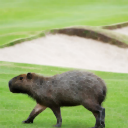
\includegraphics[scale=1.4]{./rendus/ErosionColor.png}}
\caption{Erosion de capybara.ppm}
\end{figure}

\begin{figure}[h]
\centerline{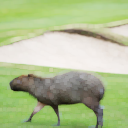
\includegraphics[scale=1.4]{./rendus/DilatationColor.png}}
\caption{Dilatation de capybara.ppm}
\end{figure}

\begin{figure}[h]
\centerline{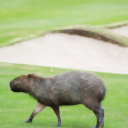
\includegraphics[scale=1.4]{./rendus/FermetureColor.png}}
\caption{Fermeture de capybara.ppm}
\end{figure}

\begin{figure}[h]
\centerline{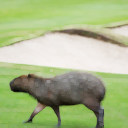
\includegraphics[scale=1.4]{./rendus/OuvertureColor.png}}
\caption{Ouverture de capybara.ppm}
\end{figure}


\end{document}